\documentclass[xcolor=dvipsnames, mathserif, handout, aspectratio=149]{beamer} 

%% auxiliary files and definitions
\usepackage{import}
\import{../aux/}{slide_layout.tex}
\import{../aux/}{definitions.tex}

%% Front page and content
\title{MS-EV0017 - Stochastic programming \& \\Robust optimisation \\[12pt]
Lecture 2/5
}
\date{\today}
\author{Fabricio Oliveira}
\institute{Department of Mathematics and Systems Analysis \\ 
           Aalto University, School of Science}

%% Begin of the file
\begin{document}

\begin{frame}[noframenumbering]
    \thispagestyle{empty}
    \titlepage
\end{frame}

\begin{frame}
%	\thispagestyle{empty}
	\frametitle{Outline of this lecture} 
	\tableofcontents
\end{frame} 

%% Slide content
\addtocounter{framenumber}{-1}
\section{Introduction}

\begin{frame}{Stochastic programming models}

	Mathematical programming models in which some of the parameters are assumed to be \alert{random variables}.	

	It comprises the following parts:
	\vspace{-6pt}
	\begin{enumerate}
		\item A mathematical programming model
		\item \alert{Deterministic} parameter values	
		\item Description of the \alert{stochasticity}, e.g.,
		\begin{itemize}
			\item a known probability distribution; 
			\item historical data;
			\item distribution properties (average, standard deviation, i.e., moments)	
		\end{itemize}
	\end{enumerate}
	
	\pause
	The most widespread use of stochastic programs relies on \alert{scenarios}:
	\vspace{-6pt}
	\begin{itemize}
		\item Lead to \alert{tractable} deterministic equivalents;
		\item Are \alert{approximations} of the original stochastic process
	\end{itemize}
	
	
	
\end{frame}

\begin{frame}{Stochastic programming models}

	 A scenario tree $\xi$ comprises \alert{sequentially observed realisations} of $\xi^t$, for $t = 1, \dots, H$:
	 \vspace{-6pt}
	 \begin{itemize}
	 	\item $\xi = (\xi^t)_{t \in [H]}$, where $(\cdot)$ denotes a \alert{sequence} and $\xi^t \in \Xi_t$;  
	 	\item a \alert{scenario} is denoted $\xi_s = (\xi_s^t)_{t \in [H]}$ forming a ``path'' through $\xi$;
	 	\item Thus, $\xi = \braces{\xi_s}_{s \in [S]}$, where $S$ is the number of scenarios.
	 \end{itemize}
	 \pause
	 
 	{\bf Example:}
 
 	\vspace{-24pt} 
 	\begin{figure}
		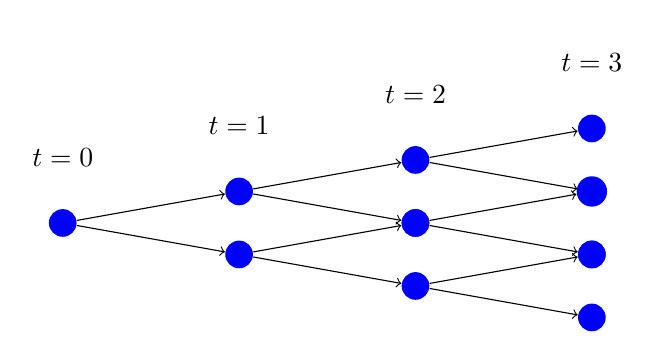
\begin{tikzpicture}[
	                   scale = 0.8, 
	                   grow = right,
	edge from parent/.style = {draw,->},
	         label distance = 2mm,
	      every node/.style = {circle, fill=blue, minimum width=1em, inner sep=1pt},
	         level distance = 28mm,
	       sibling distance = 10mm,
	                     ]
		\node[label={$t=0$}] {}
		    child {node {}
		        child {node {}
		            child {node {}}
		            child {node {}}
		                }
		        child {node {}} 
		            }
		    child {node[label={$t=1$}] {}
		        child {node {}
		            child {node {}} 
		            child {node {0}}
		                }
		        child {node[label={$t=2$}] {}
		            child {node {}} 
		            child {node[label={$t=3$}] {}}
		                }
		                };
		\end{tikzpicture}
		\vspace{9pt}
		\caption{A 4-stage (\alert{lattice}) scenario tree with 2 scenarios per stage. $\xi = (\xi^1, \xi^2, \xi^3)$;}
	\end{figure}
	
	
\end{frame}


\section{Scenario trees}


\begin{frame}{Taxonomy of scenario trees}
{Terminology}
	
	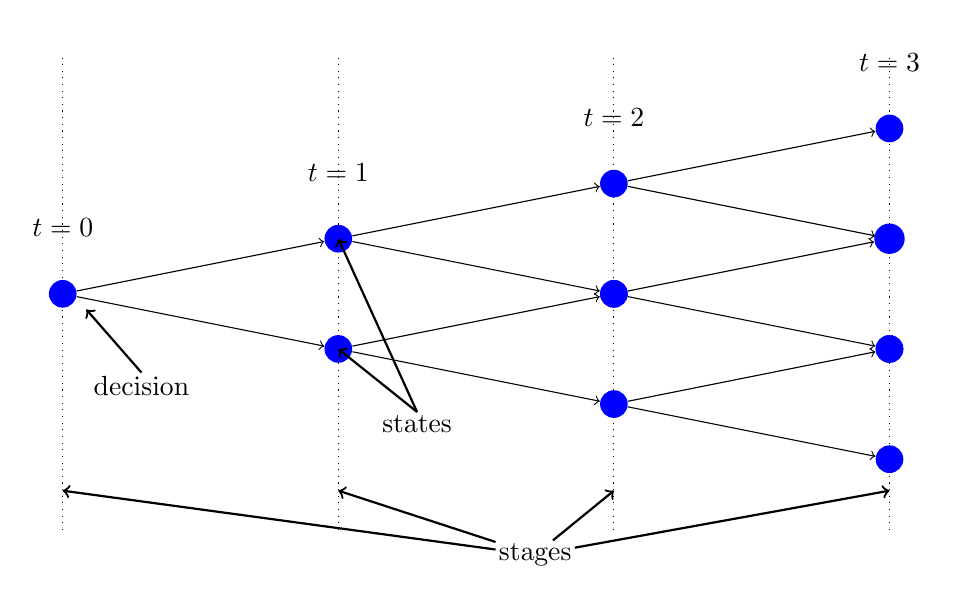
\begin{tikzpicture}[
	                   grow = right,
	edge from parent/.style = {draw,->},
	         label distance = 2mm,
	      every node/.style = {circle, fill=blue, minimum width=1em, inner sep=1pt},
	         level distance = 35mm,
	       sibling distance = 14mm,
	                     ]
	    \draw[dotted] (0,-3) -- (0,3);
		\draw[dotted] (3.5,-3) -- (3.5,3);
		\draw[dotted] (7,-3) -- (7,3);
		\draw[dotted] (10.5,-3) -- (10.5,3);
		\node[label={$t=0$}] (t0) {}
		    child {node {}
		        child {node {}
		            child {node {}}
		            child {node {}}
		                }
		        child {node {}} 
		            }
		    child {node[label={$t=1$}] (t1) {}
		        child {node {}
		            child {node {}} 
		            child {node {0}}
		                }
		        child {node[label={$t=2$}] (t2) {}
		            child {node {}} 
		            child {node[label={$t=3$}] (t3) {}}
		                }
		                };              
		 \onslide<2->{
		 \draw[->, thick] node[shape=rectangle, fill=none, below] at (1,-1) {decision} (1,-1) -- (0.3,-0.2);}
		 \onslide<3->{
		 \draw[->, thick] node[shape=rectangle, fill=none, below] at (4.5,-1.5) {states} (4.5,-1.5) -- (3.5,0.7);
		 \draw[->, thick] node[shape=rectangle, fill=none, below] at (4.5,-1.5) {} (4.5,-1.5) -- (3.5,-0.7);}
		 \onslide<4->{
		 \draw node[shape=rectangle, fill=none, above] (stages) at (6,-3.5) {stages}; 
		 \draw[->, thick] (stages) -- (0,-2.5);
		 \draw[->, thick] (stages) -- (3.5,-2.5);
		 \draw[->, thick] (stages) -- (7,-2.5);
		 \draw[->, thick] (stages) -- (10.5,-2.5);}
	\end{tikzpicture}
\end{frame}

\begin{frame}{Taxonomy of scenario trees}
	
	\begin{figure}
	\centering
	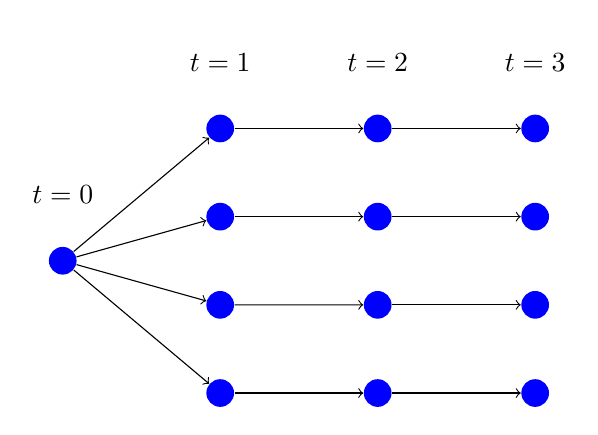
\begin{tikzpicture}[
	                   grow = right,
	edge from parent/.style = {draw,->},
	         label distance = 2mm,
	      every node/.style = {circle, fill=blue, minimum width=1em, inner sep=1pt},
	         level distance = 25mm,
	       sibling distance = 14mm,
	       scale= 0.8
	                     ]
		\node[label={$t=0$}] (t0) {}
		    child {node {} child {node {} child { node {}}}}
		    child {node {} child {node {} child { node {}}}}
		    child {node {} child {node {} child { node {}}}}
		    child {node[label={$t=1$}] {} child {node[label={$t=2$}] {} child { node[label={$t=3$}] {}}}};
    \end{tikzpicture}
    \end{figure}
    
    \alert{Branching} indicates a decision upon arrival of \alert{new information}
    \vspace{-6pt}
    \begin{itemize}
    	\item No branching, no additional information;
    	\item \alert{Fan trees} represent \alert{multi-period 2-stage problems}.
    \end{itemize}

\end{frame}


\section{Generating scenario trees}


\begin{frame}{Trade-off approximation quality vs. tractability}

	Two parameters govern the geometry of a scenario tree:
	\vspace{-6pt}
	\begin{itemize}
		\item {\bf Depth:} number of stages $H$
		\item {\bf Breadth (or width):} number of realisations per stage $|\xi^t|$
	\end{itemize}
	
	\pause
	The \alert{total of scenarios} is $O(N^{H})$ (assuming $|\xi_t| = N$ for $t \in [H]$)
	\vspace{-6pt}
	\begin{itemize}
		\item Larger $H$ convey more \alert{adaptability} to revealed information;
		\item Larger $S$ convey a more \alert{precise} description of the uncertainty;
		\item \alert{Computational tractability} issues pressure them to be as small as possible.
	\end{itemize}

	Most scenario generation methods seek to find trees with \alert{minimal $|\xi|$} such that \alert{representation quality} requirements are observed.
	
\end{frame}


\begin{frame}{Data source}

	Typical \alert{sources} for scenarios include:
	\vspace{-6pt}
	\begin{enumerate}
		\item {\bf Historical data:} past observations as possible future observations;
		\item {\bf Simulation models:} Monte Carlo, systems dynamics, agent-based and discrete event simulation;
		\item {\bf Expert elicitation:} typically a small number of scenarios with no possible (out-of-sample) testing. 
	\end{enumerate}
	
	\pause
	Often, a \alert{combination} of the above is used:
	\vspace{-6pt}
	\begin{enumerate}
		\item Start from the \alert{data};
		\item Define and fit a \alert{parametric model};
		\item Generate \alert{observations} from the model.	
	\end{enumerate}
	
\end{frame}


\begin{frame}{Scenario generation and modelling}

\begin{columns}

	\column{0.55\textwidth}
		Scenario generation must be part of \lb the \alert{modelling process}
		\begin{itemize}
			\item Problem dependent;
			\item The method for generating scenarios is a \alert{modelling decision};
			\item Often overlooked in applications;
			\item Quality of scenarios \alert{majorly} influences quality of solution (``garbage in = garbage out'').	
		\end{itemize}
	\hfil
	\column{0.45\textwidth}
		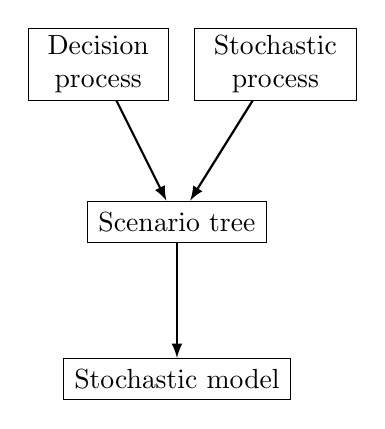
\begin{tikzpicture}
%			\draw[help lines] (0,0) grid (4,8);
			\node[draw, inner sep=1pt] (model) at (1,7) {\begin{tabular}{cc} Decision \\ process \end{tabular}};
			\node[draw, inner sep=1pt] (stoch) at (3.25,7) {\begin{tabular}{cc} Stochastic \\ process \end{tabular}};
			\node[draw, inner sep=4pt] (scen_tree) at (2,5) {Scenario tree};
			\node[draw, inner sep=4pt] (stoch_model) at (2,3) {Stochastic model};
			\draw[-latex, thick] (model) -- (scen_tree);
			\draw[-latex, thick] (stoch) -- (scen_tree);	
			\draw[-latex, thick] (scen_tree) -- (stoch_model);	
		\end{tikzpicture}
\end{columns}

	
\end{frame}


\begin{frame}{Quality measures for scenario trees}

	Apart from \alert{epistemic error} questions, two measures must be considered when generating scenario trees:
	
	\begin{enumerate}
		\item {\bf Error}
		\begin{itemize}
			\item Error introduced for using an \alert{approximation} of the real stochastic process;
			\item Unlikely to be measurable, but possible to be approximated.
		\end{itemize}
		\vfill
		\item {\bf Stability}
		\begin{itemize}
			\item Scenario-trees approximating the same stochastic process should yield the same solution;
			\item Likewise, objective function values should be \alert{stable}.
		\end{itemize}		
	\end{enumerate}
	
	\pause
	Let $\xi$ be a scenario tree representing the original \alert{stochastic process $\eta$}, and $\mathcal{F}(x, \xi) = \mathbb{E}_\xi\brackets{F(x,\xi)}$. We are interested in understanding how well
		$$
		\min_{x} \mathcal{F}(x, \xi) \text{ approximates }
		\min_{x} \mathcal{F}(x, \eta)
		$$		
	
\end{frame}


\begin{frame}{Quality measures for scenario trees}

	Let $\xi_k$, for $k=1,\dots,n$, be a collection of alternative scenario trees generated (e.g., by sampling) to represent $\eta$. We have that
	$$
		x_k^\star = \arg\min_{x} \mathcal{F}(x, \xi_k).
	$$ 
	%
	The \alert{approximation error} {\small \cite{pflug2001scenario}} is defined as 
	%
	\begin{align*}
		e(\eta, \xi_k) =~ & \mathcal{F}(\arg\min_{x} \mathcal{F}(x, \xi_k), \eta) - 	\mathcal{F}(\arg\min_{x} \mathcal{F}(x, \eta), \eta) \\
		=~ & \mathcal{F}(x_k^\star, \eta) - \min_{x} \mathcal{F}(x, \eta). 
	\end{align*}
	\pause

	\vspace{-18pt}
	\begin{itemize}
		\item Calculating $\mathcal{F}(x_k^\star, \eta)$ requires evaluating the ``true'' objective function;
		\item Alternatively, \alert{Monte Carlo simulation} is often employed to approximate $\mathcal{F}(x_k^\star, \eta)$;
		\item Clearly, there is no way to evaluate $\min_{x} \mathcal{F}(x, \eta)$.
	\end{itemize}

\end{frame}


\begin{frame}{Stability for scenario trees}{Out-of-sample stability} 

	Assume that we can \alert{approximate} $\mathcal{F}(x_k^\star, \eta)$. This allows us to
	\vspace{-6pt}
	\begin{itemize}
		\item compare solutions $x_{1}^\star$ and $x_{2}^\star$;
		\item compare \alert{alternative} scenario generation methods;
		\item perform \alert{out-of-sample} stability test:
		\begin{enumerate}
			\item Generate a set of scenario trees $\braces{\xi_1, \dots, \xi_n}$;
			\item Obtain solutions $x_k$, $k=1,\dots,n$;	
			\item Test whether $\mathcal{F}(x_k^\star, \eta) \approx \mathcal{F}(x_l^\star, \eta), \text{ for } k,l = 1\dots, n : k \neq l$.
		\end{enumerate}
	\end{itemize}
	
	\pause
	{\bf Remarks:}
	\vspace{-6pt}
	\begin{itemize}
		\item $e(\eta, \xi_k) \approx 0 \Rightarrow e(\eta, \xi_k) \approx e(\eta, \xi_l) \equiv \mathcal{F}(x_k^\star,\eta) \approx \mathcal{F}(x_l^\star,\eta)$;
		\item The procedure above can also be used to \alert{assess scenario tree} width (scenarios per stage).
	\end{itemize}
	
\end{frame}



\begin{frame}{Stability for scenario trees}{In-sample stability}

	\alert{In-sample} stability is defined as
	$$
		\mathcal{F}(x_k^\star, \xi_k) \approx \mathcal{F}(x_l^\star, \xi_l), \text{ for } k,l = 1,\dots, n : k \neq l.
	$$
	
	\pause
	In some contexts, can also be defined as
	$$
		||x_k^\star - x_l^\star||_p \approx 0, \text{ for } k,l = 1,\dots, n : k \neq l.
	$$
	where $|| \cdot ||_p$ is a vector $p$-norm.
	
	\pause
	\begin{itemize}
		\item No direct connection to \alert{out-of-sample} stability;
		\item Useful for assessing the \alert{internal} stability of a random scenario generation method;
		\item Translates into \alert{confidence} in the objective function value reported.
	\end{itemize}
	
\end{frame}

\begin{frame}{Stability for scenario trees}{Final considerations}
	Some practical advice:
	\begin{itemize}[<+->]
		\item No stability implies \alert{dependence} on the scenario tree. To improve stability one can
		\begin{enumerate}
			\item Consider alternative scenario generation methods
			\item Increase the number of scenarios	
		\end{enumerate}
		\item In case approximating $\mathcal{F}(x_k^\star, \eta)$ is not feasible, cross-testing can be employed. Let 
		$$
			\overline{\mathcal{F}} = \braces{\mathcal{F}(x_k^\star, \xi_l)}_{k,l = 1,\dots, n : k \neq l}.
		$$
		Out-of-sample stability implies that the standard deviation of $\overline{\mathcal{F}}$ is close to 0.
		\item For a rigorous treatment of stability, check {\small \cite{dupavcova1990stability, schultz2000some, heitsch2006stability}}.
	\end{itemize}
\end{frame}

\begin{frame}{Stability for scenario trees {\small \cite{dillon2017two}}}
	\centering
	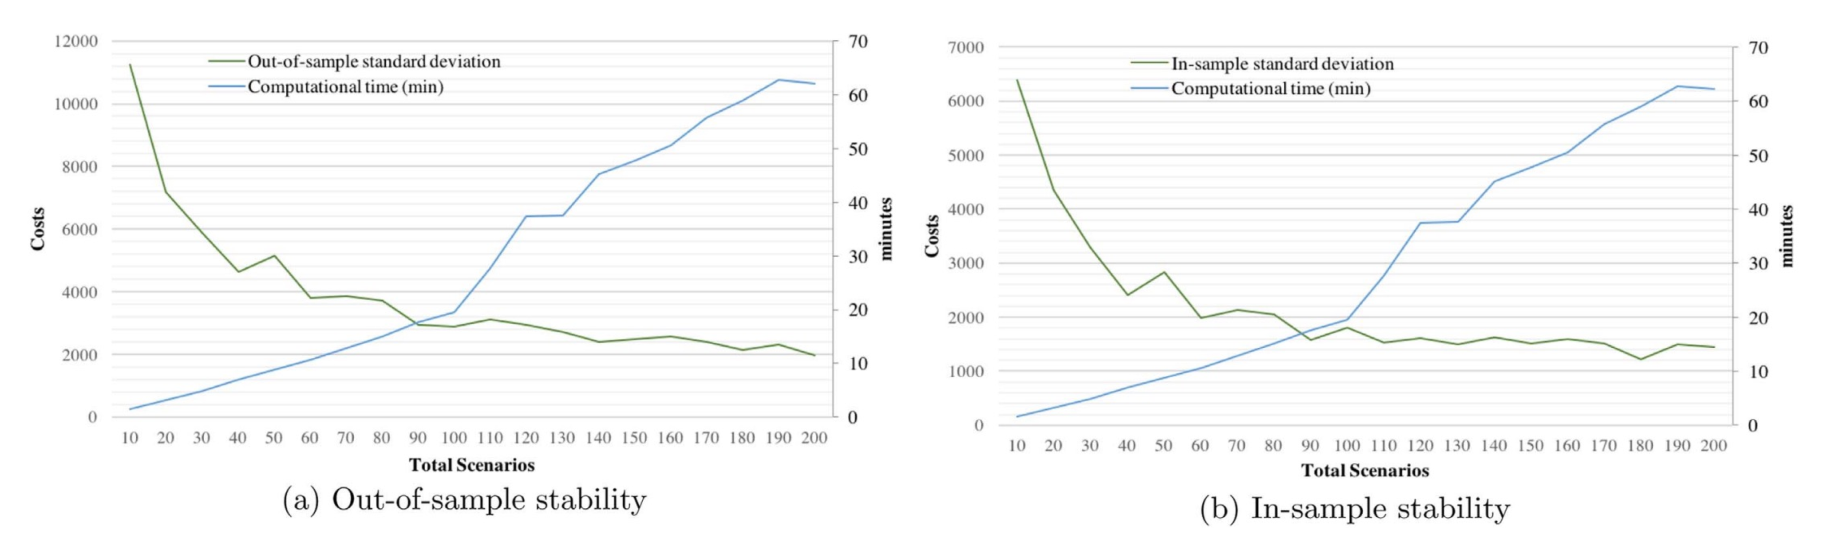
\includegraphics[width=1\textwidth]{figures/scen_stability.pdf}
	
\end{frame}



\section{Scenario (tree) generation methods}


\begin{frame}{Scenario generation methods}

	The main types of scenario-generation methods are:
	\begin{enumerate}[<+->]
		\item {\bf Sampling:} Monte-Carlo sampling, or quasi Monte-Carlo sampling using variance reduction techniques (e.g., Sobol sequences). Combined with Sample Average Approximation (SAA). 
		\item {\bf Moment matching:} artificially generates a set of scenarios with the same (four plus correlation, usually) moments as the desired distribution;
		\item {\bf Metric-based:} form smaller scenario sets whilst minimising some probabilistic distance metric. Includes clustering (k-means and related methods) and scenario reduction. %(\alert{Dupacova et al. 2003, Heitsch and Romisch, 2003})
	\end{enumerate}

	
\end{frame}

\begin{frame}{Scenario generation methods}{Moment matching}

	Build a scenario tree $\xi = \braces{(z_s,p_s)}_{s \in [S]}$ that has \alert{statistical moments} $f_m(z,p)$ matching $M^{\text{VAL}}_m$ \alert{target} values.
	\begin{itemize}
		\item Moments extracted from the original distribution, or data;
		\item The following problem must be solved ({\small \cite{hoyland2001generating}}):
		\begin{equation*}
			\begin{aligned}
				\min_{z, p \ge 0} & \sum_{m \in M} w_m(f_m(z,p) - M^{\text{VAL}}_m)^2 \\
				\text{s.t.:~} & \sum_{j=1}^{S} p_j = 1,	
			\end{aligned}
		\end{equation*}
		where $w_m$ are weights.
	\end{itemize}
	
	{\bf Remark:} \alert{\small \cite{hoyland2003heuristic}} show how the above problem can be heuristically solved.
\end{frame}

\begin{frame}{Scenario generation methods}{Metric-based methods}

	Probability-metric based methods use the following result {\small \cite{pflug2001scenario}}
	%
	\begin{equation*}
		e(\eta, \xi_k) \le K d(\eta, \xi_k)	
	\end{equation*}
	%
	where $K$ is a (Lipschitz-related) constant and $d$ is a \alert{Wasserstein distance} between $\eta$ and $\xi_k$. Thus, the focus is on obtaining trees that \alert{minimise} $d$.

	\pause
	Let $\xi^l = (z^l, p^l) \in \Xi^l$. The ($p$-order) Wasserstein distance $d(\xi^1,\xi^2)$ is given by:

	\vspace{6pt}
	\begin{columns}
	\column{0.45\textwidth}
	\begin{equation*}
		\begin{aligned}
			\mini_{\pi} & \sum_{i \in \xi^1, j \in \xi^2} ||z^1_i - z^2_j||_p \pi_{ij} \\
			\st & \sum_{j \in \xi^2} \pi_{ij} = p^1_i, \ \forall i \in \xi_1 \\ 
						  & \sum_{i \in \xi^1} \pi_{ij} = p^2_j, \ \forall j \in \xi_2.
		\end{aligned}
	\end{equation*}
	\column{0.45\textwidth}
	
	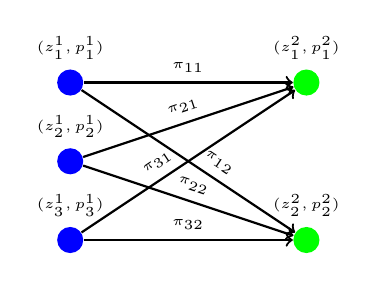
\begin{tikzpicture}
%		\draw[help lines] (0,0) grid (3,3);
		\node[circle, fill= blue, label={\tiny $(z_1^1, p_1^1)$}] (1) at (0,2) {};
		\node[circle, fill= blue, label={\tiny $(z_2^1, p_2^1)$}] (2) at (0,1) {};
		\node[circle, fill= blue, label={\tiny $(z_3^1, p_3^1)$}] (3) at (0,0) {};
		\node[circle, fill= green, label={\tiny $(z_1^2, p_1^2)$}] (4) at (3,2) {};
		\node[circle, fill= green, label={\tiny $(z_2^2, p_2^2)$}] (5) at (3,0) {};
		\draw[thick, ->] (1) edge node [sloped, above] {\tiny $\pi_{11}$} (4);
		\draw[thick, ->] (2) edge node [sloped, above] {\tiny $\pi_{21}$} (4);
		\draw[thick, ->] (3) edge node [sloped, above left] {\tiny $\pi_{31}$} (4);
		\draw[thick, ->] (1) edge node [sloped, above right] {\tiny $\pi_{12}$} (5);
		\draw[thick, ->] (2) edge node [sloped, above] {\tiny $\pi_{22}$} (5);
		\draw[thick, ->] (3) edge node [sloped, above] {\tiny $\pi_{32}$} (5);
	\end{tikzpicture}
	\end{columns}

\end{frame}

\begin{frame}{Scenario generation methods}{Metric-based methods}
	
		{\color{blue}1.} {\bf ``Clustering-like'' methods:}
		\begin{itemize}
			\item $k$-means, and variants incorporating Wasserstein distance as the metric {\small \cite{condeixa2020wasserstein}}
			\item Work well in case scenarios are generated from \alert{data} {\small\cite{kaut2021scenario}};
			\item {\small \cite{lohndorf2016empirical}}: \alert{Learning-based algorithms} such as competitive learning and Voronoi cell sampling as alternatives to $k$-means. 
		\end{itemize}
		\vspace{-6pt}
		\begin{figure}
		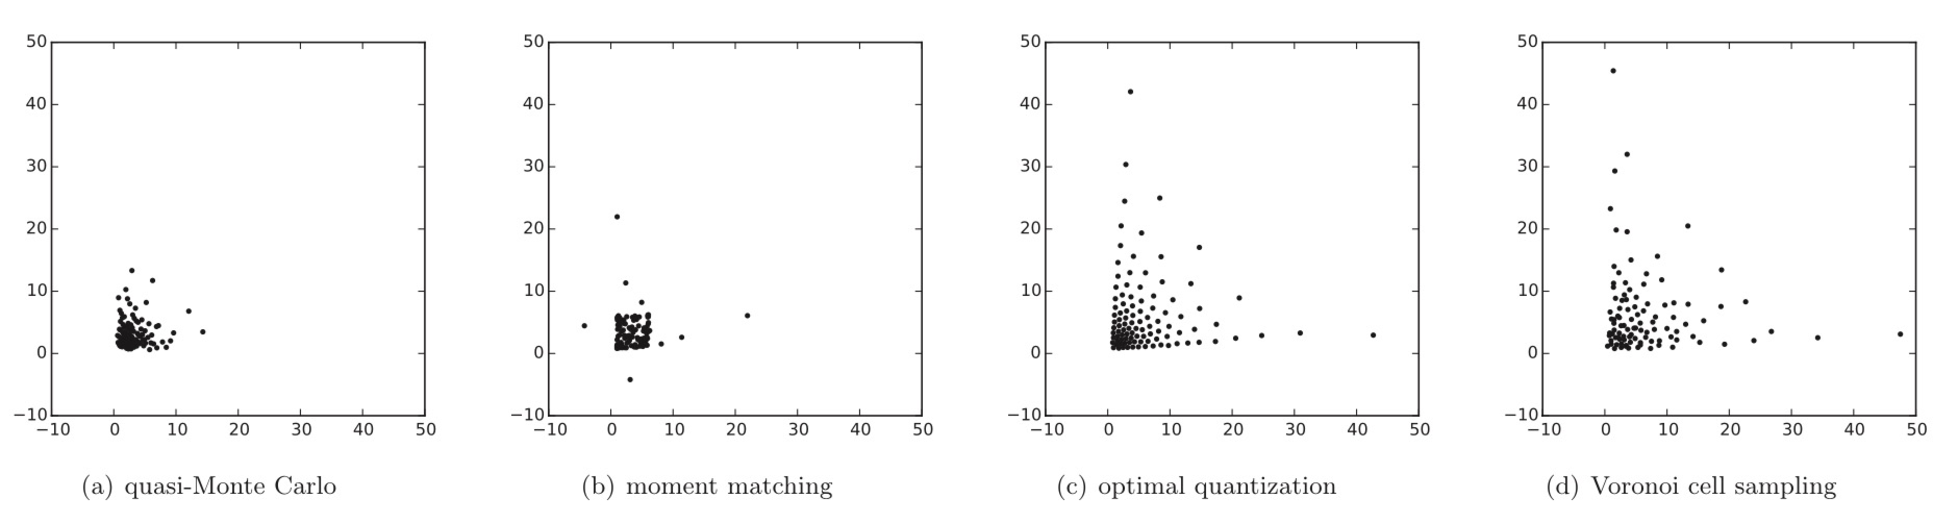
\includegraphics[width=\textwidth]{figures/scen_methods(Lohndorf).pdf}
		\caption{comparison of scenario generation methods (\cite{lohndorf2016empirical})}			
		\end{figure}
	
\end{frame}

\begin{frame}{Scenario generation methods}{Metric-based methods}

		{\color{blue}2.} {\bf Scenario reduction methods:} Obtain $\xi^2$ from $\xi^1$ where $|\xi^2| < |\xi^1|$.
		\begin{itemize}
			\item Based on the theory of stability of stochastic programs {\small \cite{romisch2003stability}}
			\begin{itemize}
				\item Changes in the solution can be approximated using a Fortet-Mourier-type metric
				\item Calculation leads to a Monge-Kantorovich mass transportation problem
			\end{itemize}	
			\onslide<2->{
			\item ``Historical'' chronology:
			\begin{enumerate}
				\item {\small \cite{dupavcova2003scenario, heitsch2003scenario}}: first \alert{backward reduction} and \alert{forward selection} methods;
				\item {\small \cite{heitsch2007note}} improved versions of the heuristics;
				\item \cite{heitsch2009scenario} The above does not work for \alert{multi-stage} problems. Provides a method that does.  
			\end{enumerate}}
		\end{itemize}

\end{frame}

\begin{frame}{Scenario generation methods}{Scenario reduction}

	Types of reduction algorithms. Let $K$ be a target value for $|\xi^2|$
	\vspace{-6pt}
	\begin{itemize}
		\item {\bf Backward reduction:} repeat until $|\xi^2|=K$. Start from $\xi^1$ 
		\begin{enumerate}
			\item Find the scenario whose removal causes the \alert{smallest error increase}
			\item Remove the scenario and redistribute its probability
		\end{enumerate} 
		\item {\bf Forward selection:} repeat until $|\xi^2|=K$. Start from $\xi^2 = \emptyset$
		\begin{enumerate}
			\item Find the scenario whose inclusion causes the \alert{largest error decrease}
			\item Add the scenario and redistribute its probability
		\end{enumerate} 
	\end{itemize}
	
	\pause
	Some final practical remarks:
	\vspace{-6pt}
	\begin{itemize}
		\item In {\small \cite{heitsch2003scenario}}, their results indicate:
		\begin{itemize}
			\item 50\% of the scenarios gives 90\% relative accuracy
			\item 1\% of the scenarios gives 50\% accuracy
		\end{itemize}
		\item \alert{Forward selection} gives better results, but is slow for large $|\xi^1|$ and $K$.
		\item \alert{Scenred2} (GAMS) is an available implementation.		
	\end{itemize} 
	
\end{frame}

\begin{frame}{Scenario generation methods}{Some of my own experience}
	\begin{figure}
		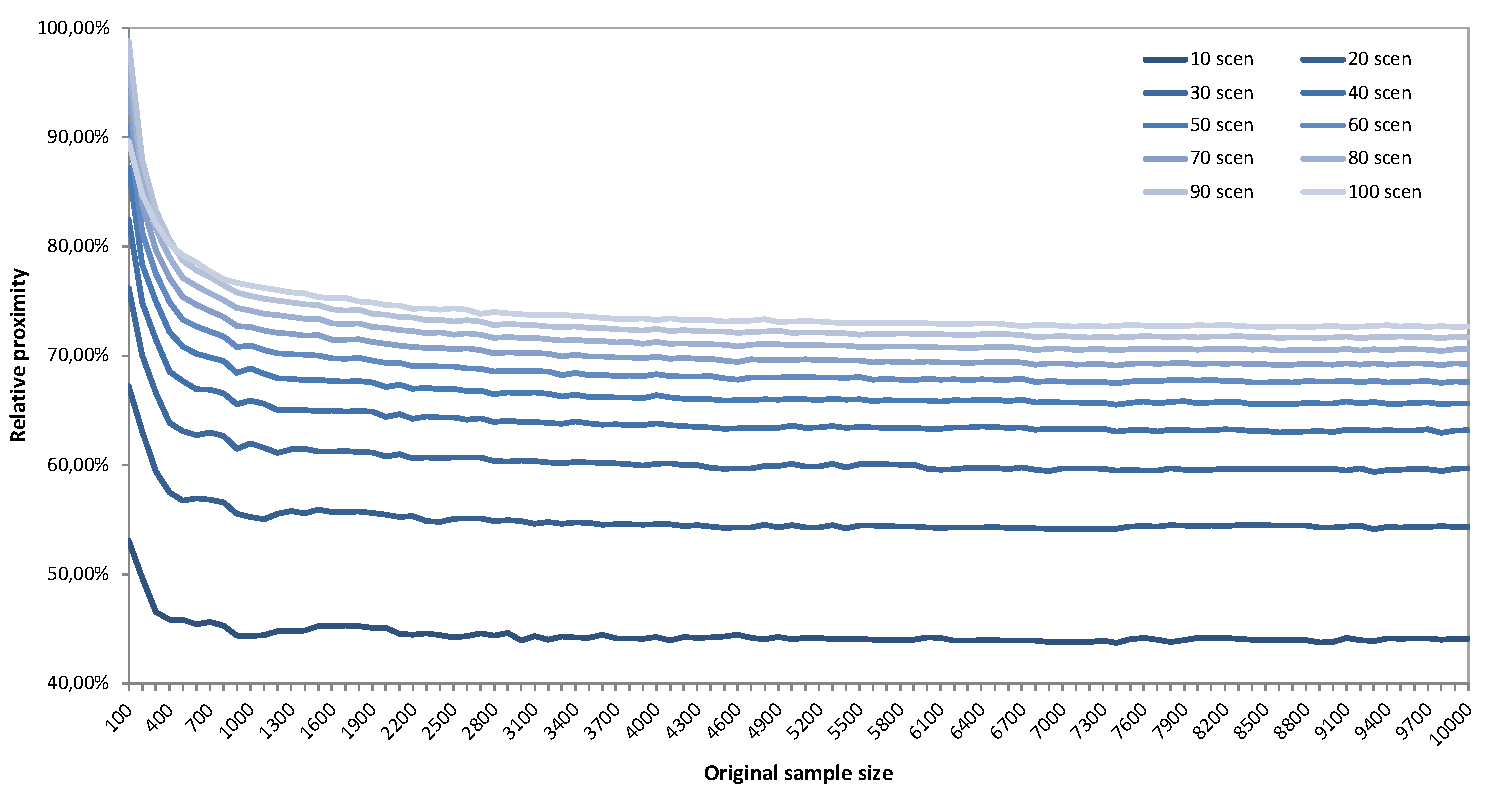
\includegraphics[width=0.95\textwidth]{figures/scenred.pdf}
		\caption{Relative accuracy for scenario reduction; $x$-axis is $|\xi^1|$, lines are different $|\xi^2|$. \cite{oliveira2016framework}}	
	\end{figure}

\end{frame}

\begin{frame}{Scenario generation methods}{Some of my own experience}

	
	%
	\begin{figure}
		\begin{subfigure}{0.45\textwidth}
			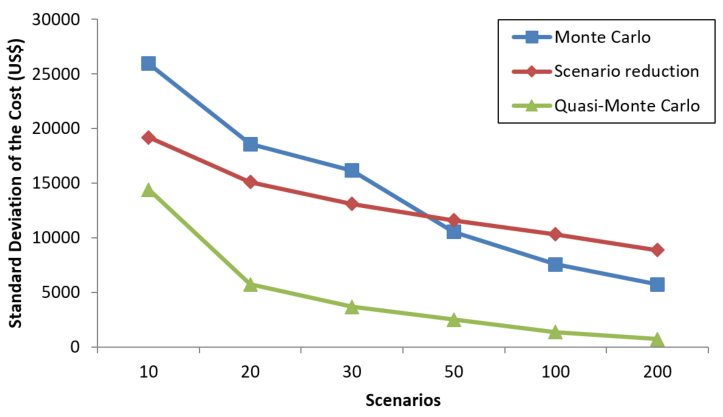
\includegraphics[width=1.05\textwidth]{figures/stdev_cost_in.pdf}
			\caption{In-sample}
		\end{subfigure}
		\hfill
		\begin{subfigure}{0.45\textwidth}
			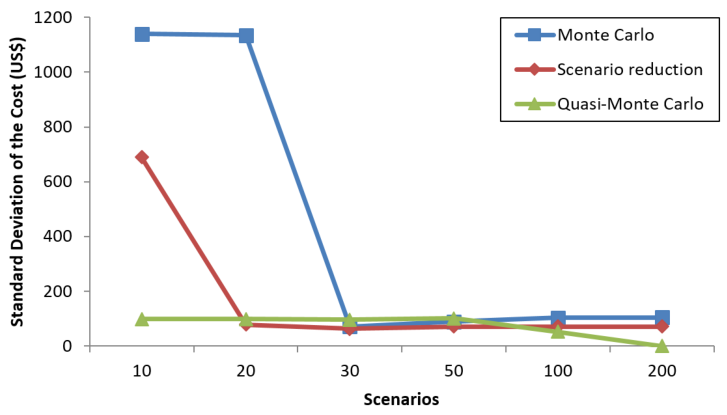
\includegraphics[width=1.05\textwidth]{figures/stdev_cost_out.pdf}
			\caption{Out-of-sample}
		\end{subfigure}
		\caption{Objective function standard deviation comparing 3 alternative scenario reduction methods. Original sample had 1000 scenarios \cite{fernandez2018optimizing}}	
	\end{figure}



	
\end{frame}



\section{Sample Average Approximation (SAA)}

	
\begin{frame}{What is SAA}

	SAA {\small \cite{shapiro1998simulation}} is an \alert{alternative} to generating scenario trees in the context of stochastic programming
	
	\begin{columns}
		\column{0.45\textwidth}
		\begin{itemize}
			\item Purely based on \alert{sampling};
			\item Monte Carlo simulation for estimating objective function bounds;
			\item Useful for handling \alert{large} scenario sets;
			\item The sample $m$ scenario tree size $N$ is such that $N << |\xi|$ or $|\eta|$;
			\item Requires solving $M$ problems.
		\end{itemize}

		\column{0.5\textwidth}
		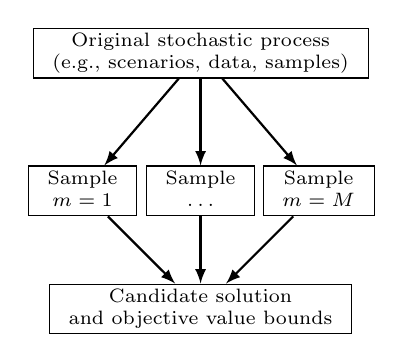
\begin{tikzpicture}
%		    \draw[help lines] (0,0) grid (4,8);
			\node[draw, inner sep=1pt] (original) at (2,7) {\scriptsize \begin{tabular}{cc} Original stochastic process \\ (e.g., scenarios, data, samples) \end{tabular}};
			\node[draw, inner sep=1pt] (sample1) at (0.5,5.25) {\scriptsize \begin{tabular}{cc} Sample \\ $m=1$ \end{tabular}};
			\node[draw, inner sep=1pt] (sample2) at (2,5.25) {\scriptsize \begin{tabular}{cc} Sample \\ $\dots$ \end{tabular}};
			\node[draw, inner sep=1pt] (sample3) at (3.5,5.25) {\scriptsize \begin{tabular}{cc} Sample \\ $m=M$ \end{tabular}};
			\node[draw, inner sep=1pt] (SAA) at (2,3.75) {\scriptsize \begin{tabular}{cc} Candidate solution \\ and objective value bounds \end{tabular}};
			\draw[-latex, thick] (original) -- (sample1);
			\draw[-latex, thick] (original) -- (sample2);
			\draw[-latex, thick] (original) -- (sample3);
			\draw[-latex, thick] (sample1) -- (SAA);
			\draw[-latex, thick] (sample2) -- (SAA);
			\draw[-latex, thick] (sample3) -- (SAA);
		\end{tikzpicture}
	\end{columns}

	
\end{frame}


\begin{frame}{How SAA works}

	SAA is based on the \alert{law of large numbers} (LLN) and the \alert{central limit theorem} (CLT). As such, we can
	\vspace{-6pt} 
	\begin{itemize}
		\item Estimate bounds using mean values;
		\item Estimate confidence intervals.
	\end{itemize}
	
	\pause 
	First, let us define our notation for \alert{2SSP}s
	\begin{equation*}
		z = \min_x f(x), 	
	\end{equation*}
	where: 
	\begin{itemize}
		\item $f(x) = \mathbb{E}_\xi\brackets{F(x, \xi)}$%
		%
		\footnote{$f(x)$ is a shorthand for $\mathcal{F}(x,\xi)$.}
		%
		\item $F(x,\xi) = \braces{c^\top x + Q(x,\xi) : x \in X}$;
		\item $Q(x, \xi) = \mini_y \braces{q(\xi)^\top y : W(\xi)y = h(\xi) - T(\xi)x, y \ge 0}$;
		\item $X=\braces{x \in \reals^n : Ax = b, x \ge 0}$.	
	\end{itemize}
	
\end{frame}


\begin{frame}{How SAA works}{Calculating a lower bounds for $z$}

	Let $N$ be the number of samples we draw from our original stochastic process, forming the \alert{scenario tree} $\xi = \braces{\xi_1, \dots, \xi_N}$.
	
	Then, we can solve the \alert{sample-based approximation} problem
	\begin{equation}
		\hat{z}_N = \min_x \braces{\tilde{f}_N(x) = \frac{1}{N}\sum_{n=1}^N F(x,\xi_n)}.
	\end{equation}
	
	\pause
	First, notice that $\tilde{f}_N(x)$ is an \alert{unbiased estimator}%
	%
	\footnote{LLN: $\lim_{N \rightarrow \infty} \mathbb{E}\brackets{\frac{\sum_{n=1}^N X_n}{N}} = \frac{N \overline{X}}{N} = \overline{X}$ for i.i.d. random variable $X_n$ with mean value $\overline{X}$. \label{fn:unbiased_estimator}} 
	%
	for $f(x)$:
	\begin{equation*}
		\mathbb{E}_\xi\brackets{\tilde{f}_N(x)} = \frac{1}{N}\mathbb{E}_\xi\brackets{\sum_{n=1}^N F(x,\xi_n)} \xrightarrow{LLN} \frac{1}{N} (Nf(x)) = f(x).	\qed
	\end{equation*}

\end{frame}



\begin{frame}{How SAA works}{Calculating lower bounds for $z$}

	We now show that $\mathbb{E}\brackets{\hat{z}_N}$ is a \alert{lower bound} on $z$:
	%
	\begin{align*}
		\hat{z}_N = &\min_x \braces{\frac{1}{N}\sum_{n=1}^{N}F(x, \xi_n)} \le \frac{1}{N}\sum_{n=1}^{N}F(x, \xi_n) \\
		 &\mathbb{E}_\xi\brackets{\min_x \braces{\frac{1}{N}\sum_{n=1}^{N}F(x, \xi_n)}} \le  \mathbb{E}_\xi\brackets{\frac{1}{N}\sum_{n=1}^{N}F(x, \xi_n)} \\
		 &\mathbb{E}_\xi\brackets{\hat{z}_N} \le  \mathbb{E}_\xi\brackets{\frac{1}{N}\sum_{n=1}^{N}F(x, \xi_n)} \\ 
		 &\mathbb{E}_\xi\brackets{\hat{z}_N} \le \min_x \braces{\mathbb{E}_\xi\brackets{\frac{1}{N}\sum_{n=1}^{N}F(x, \xi_n)}} \xrightarrow{N \rightarrow \infty} \\ 
		 & \quad\quad\quad\quad \min_x \braces{\mathbb{E}_\xi\brackets{F(x,\xi)}} = \min_x f(x) = z. \qed
	\end{align*}
	
\end{frame}


\begin{frame}{How SAA works}{Calculating lower bounds for $z$}

	In turn, we can approximate $\mathbb{E}\brackets{\hat{z}_N}$ using \alert a \alert{sample estimate}.
	
	\begin{enumerate}[<+->]
		\item For that, we sample $M$ scenario trees of size $N$: 	
		$$
			\braces{\xi_1^1,\dots,\xi_N^1}, \dots, \braces{\xi_1^M,\dots,\xi_N^M}.
		$$
		\item For each scenario tree, we solve 
		\begin{equation*} 
			\hat{z}^m_N = \min_x\braces{\frac{1}{N}\sum_{n=1}^{N}F(x, \xi_n^m)}
		\end{equation*}
		\item We can then estimate%
		\footnote{Again an unbiased estimator, see footnote \ref{fn:unbiased_estimator}.} 
		%
		 $\mathbb{E}\brackets{\hat{z}_N}$ as
		\begin{equation*}
			L_N^M = \frac{1}{M} \sum_{m=1}^M \hat{z}^m_N.
		\end{equation*}
	\end{enumerate}
	
\end{frame}


\begin{frame}{How SAA works}{Statistical bounds for $L_N^M$}

	We can use the CLT to provide \alert{confidence intervals} for $L_N^M$. A sample-estimate for $\sigma^2_{L_N^M}$ can be obtained as 
	$$
		s^2_{L_N^M} = \frac{1}{M-1}	\sum_{m=1}^M (\hat{z}^m_N - L_N^M)^2.
	$$
	\pause
	We can use $s^2_{L_N^M}$ to obtain an  \alert{1-$\alpha$ confidence interval} for $L_N^M$:
	$$
		\brackets{L_N^M - \frac{z_{\alpha/2} s_{L_N^M}}{\sqrt{M}}, L_N^M + \frac{z_{\alpha/2} s_{L_N^M}}{\sqrt{M}}}
	$$
	where $z_{\alpha/2}$ is the standard normal $1-\alpha/2$ quantile.
	
\end{frame}


\begin{frame}{How SAA works}{Calculating upper bounds for $z$}

	Let 
	$$
		\hat{x}^m_N = \argmin_x\braces{\frac{1}{N}\sum_{n=1}^{N}F(x, \xi_n^m)}, \ \forall m \in [M].
	$$
	Under a relatively complete recourse assumption, we have that $f(\hat{x}^m_N) \ge z$, $\forall m \in [M]$. 
	
	\pause 
	We can obtain an unbiased estimate for \alert{$f(\hat{x}^m_N)$} by
	\begin{enumerate}
		\item \alert{Choosing} one solution $\hat{x}^{m'}_N$, $m' \in [M]$;
		\item Sampling $T$ scenario trees of size $\overline{N}$
		$$
			\braces{\xi_1^1, \dots \xi_{\overline{N}}^1}, \dots, \braces{\xi_1^T, \dots \xi_{\overline{N}}^T}
		$$
		\item For each scenario tree $t$, we evaluate
		\vspace{-3pt}
		$$
			\check{z}_{\overline{N}}^t = \frac{1}{\overline{N}} \sum_{n=1}^{\overline{N}} F(\hat{x}^{m'}_N, \xi_n^t)
		$$
	\end{enumerate}
	
\end{frame}


\begin{frame}{How SAA works}{Calculating upper bounds for $z$}

	\begin{enumerate}
		\item[4.] We can estimate $f(\hat{x}^m_N)$ as
		\begin{equation*}
			U_{\overline{N}}^T = \frac{1}{T} \sum_{t=1}^T \check{z}_{\overline{N}}^t.
		\end{equation*}
	\end{enumerate}
	
	Analogously, we can use the sample-estimate for $\sigma_{U_{\overline{N}}^T}^2$
	$$
		s^2_{U_{\overline{N}}^T} = \frac{1}{T-1}	\sum_{t=1}^T (\check{z}_{\overline{N}}^t - U_{\overline{N}}^T)^2
	$$
	to calculate the \alert{1-$\alpha$ confidence interval} for $U_{\overline{N}}^T$ as
	$$
		\brackets{U_{\overline{N}}^T - \frac{z_{\alpha/2} s_{U_{\overline{N}}^T}}{\sqrt{T}}, U_{\overline{N}}^T + \frac{z_{\alpha/2} s_{U_{\overline{N}}^T}}{\sqrt{T}}}.
	$$
	
\end{frame}


\begin{frame}{On estimating optimality gaps}

	In this context, an \alert{optimality gap} refers to the quantity
	$$
		f(\hat{x}^{m'}_N) - z.
	$$
	
	\pause
	On the other hand, we know that
	$$
		  \mathbb{E}\brackets{\hat{z}_N} \le z \le f(\hat{x}^{m'}_N).
	$$
	Since we have estimates for $\mathbb{E}\brackets{\hat{z}_N}$ ($L_N^M$) and $f(\hat{x}^{m'}_N)$ ($U_{\overline{N}}^T$), we can calculate the \alert{optimality gap} estimate
	\begin{equation*}
		gap(N,M,\overline{N},T) = U_{\overline{N}}^T - L_N^M.
	\end{equation*}
	
	\pause
	Confidence intervals can also be obtained for $gap(N,M,\overline{N},T)$ using   
	$$
		\sigma^2_{gap(N,M,\overline{N},T)} = s^2_{L_N^M} + s^2_{U_{\overline{N}}^T}.
	$$ 
	

\end{frame}



\begin{frame}{On estimating optimality gaps}

Some remarks on $gap(N,M,\overline{N},T)$:
	\begin{itemize}[<+->]
		\item $gap(N,M,\overline{N},T)$	is a \alert{biased} estimator, since 
		$$
			f(\hat{x}^{m'}_N) - \mathbb{E}\brackets{\hat{z}_N} \ge f(\hat{x}^{m'}_N) - z;
		$$
		\item As it overestimates $f(\hat{x}^{m'}_N) - z$, it is still useful in practice;
		\item Confidence intervals for $gap(N,M,\overline{N},T)$ can be \alert{improved} by reducing:
			\begin{enumerate}
				\item $s^2_{L_N^M}$, via increasing $N$ and $M$: larger $N$ leads to larger problems, but they can be solved as $M$ \alert{parallel} problems;
				\item $s^2_{U_{\overline{N}}^T}$	, via increasing $\overline{N}$ and $T$; larger $\overline{N}$ leads to more costly evaluation; solvable as $T$ (as $\overline{N} \times T$ for 2SSPs) parallel problems.
			\end{enumerate}
	\end{itemize}	
\end{frame}


\begin{frame}{Final practical remarks}
	\begin{columns}
	\column{0.5\textwidth}
	Regarding choosing a solution $\hat{x}^{m'}_N$:
	\begin{itemize}
		\item If feasible, evaluate all distinct solutions $\hat{x}^{m}_N$ for $m \in \brackets{M}$ and choose that with \alert{best} $L_N^M$, $U_{\overline{N}}^T$ or $gap(N,M,\overline{N},T)$;
		\item Too many \alert{distinct} solutions may indicate that $N$ is too \alert{small}. Perform stability analysis.
		\item SAA holds for \alert{non-independent} sampling schemes (e.g., Latin hypercube sampling or quasi Monte Carlo). These help keep $N$ small.
	\end{itemize}
	
	\pause
	\column{0.47\textwidth}
	\vspace{-12pt}
	\begin{figure}
	    \centering
	    \includegraphics[width=0.65\textwidth]{figures/Monte_carlo.pdf}
		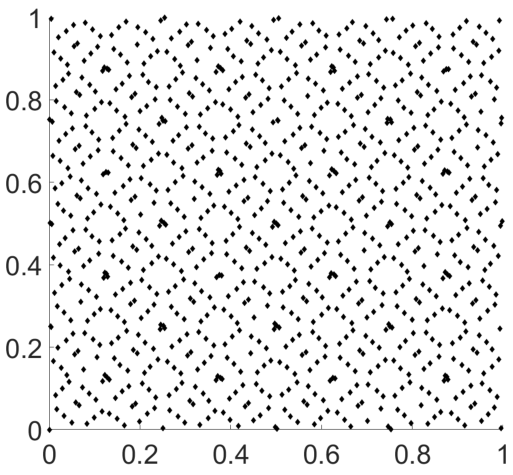
\includegraphics[width=0.65\textwidth]{figures/quasi_mc.pdf}	
		\caption{Monte Carlo (top) and quasi-Monte Carlo (bottom) sampling {\small \cite{fernandez2018optimizing}}}
	\end{figure}
		
	\end{columns}
	
\end{frame}


\begin{frame}{Final practical remarks}
	Regarding the choice of $N$ {\small \cite{oliveira2012optimization}}:
	\begin{itemize}[<+->]
		\item Notice that $\hat{z}_N$ is the expected value of the \alert{random variable}
		$$
			z_N(\xi) = F(\hat{x}_N, \xi), \text { where } \hat{x}_N = \argmin_x \braces{\frac{1}{N}\sum_{n=1}^N F(x,\xi_n)}
		$$
		\item As such, we can estimate its sample-based variance and a $1-\alpha$ confidence interval, given by
		$$
			s_N^2 = \frac{1}{N-1}\sum_{n=1}^N (\hat{z}_N - z_N(\xi_n))^2 \text{ and } \hat{z}_N \pm \frac{z_{\alpha/2} s_N}{\sqrt{N}}.
		$$
		\item If we predefine a desired \alert{relative width} $\beta$ for the confidence interval, we can infer that
		$$
			N \ge \left(\frac{z_{\alpha/2}s_N}{(\beta/2)\hat{z}_N}\right)^2.
		$$
		
	\end{itemize}
	
\end{frame}


\begin{frame}{Tutorial 3}

\centering
\large
\bf 
SAA example

	
\end{frame}


\begin{frame}[allowframebreaks]{References}
	\bibliographystyle{apalike}
	\bibliography{../aux/references.bib}
\end{frame}




\end{document}